% Results. Part 1 is Martin's text, generated from Martin/results_part1.md by report/md2tex.py.
% Part 2 is Diego's (with Claude), from Diego/d2_labelling/RESULTS.md and Diego/d5_classifier/results.txt.
% Part 3 is Anas's (with Claude): sections/results_part3.tex, a copy of Anas/results_part3.tex (edit there and copy),
% followed by Martin's M6 paragraph. Full length on purpose for the 25 Nov read-through.

\section*{Results}

\subsection*{Two maps of the same House}
% Generated by report/md2tex.py from Martin/results_part1.md. Do not edit by hand.
\textbf{Two maps of the same House.} We built two networks on the same 450 Republicans and Democrats of the 119th House. In the \emph{working map}, two members are tied if one cosponsored a bill or joint resolution that the other sponsored (46,513 ties). In the \emph{floor map}, two members are tied if one named the other in a floor speech, leaving out yields of debate time (3,970 ties from 8,469 mentions; Methods).

\textbf{The floor map is less divided by party than the working map.} 38.7\% of floor ties cross the aisle (Fig.~1\emph{A} and \emph{C}). The floor map is about twelve times sparser, so we compare it with working ties drawn at random at the same size: across 200 draws, 28.6\% of working ties cross the aisle (range 26.8\% to 30.6\%), and no draw comes within eight points of the floor map (Fig.~1\emph{B} and \emph{C}). Party modularity agrees: 0.112 for the floor map against 0.211 (0.193 to 0.230) for the draws (Fig.~1\emph{D}). Leaving out yields does not create the gap: with yields kept, the floor map is at 35.2\% against 28.7\%. Members' strongest working partnerships are far more partisan still: of the 3,970 pairs who share the most bills, 12.8\% cross the aisle.

\textbf{Both maps are more divided than chance, and the floor map's division is partly procedure.} If ties were rewired at random with every member keeping their number of ties, about half would cross the aisle and modularity would be near zero in both maps (Fig.~1\emph{C} and \emph{D}). Floor debate has a structure of its own: each debate has a cast, often with a manager from each party. Shuffling who is named only within each debate leaves a modularity of 0.074 (0.065 to 0.082 over 200 shuffles) against 0.112 observed. The debates thus account for about two thirds of the floor map's party division; the rest, members naming their own side beyond what the debate forces, exceeds every shuffle. State delegations account for almost none of it: keeping each member's number of ties within their own state gives a modularity of 0.001 (at most 0.023 over 200 draws).

\textbf{Communities follow party on one map and committees on the other.} On the working map, Louvain's communities are the two parties (normalised mutual information with party, NMI, 0.83). On the floor map they cut across party (NMI 0.03, against 0.29 for working draws of the same size): eight communities of 28 to 80 members, each holding both parties. In seven of them one House committee is 3.0 to 7.9 times as common as in the House as a whole, among them Appropriations (82\% of the community's members), Ways and Means (79\%) and Energy and Commerce (67\%); the eighth gathers the party leaders. 44\% of floor ties join two members of the same committee, against 17.1\% when ties are rewired at random, and so do 50\% of cross-party floor ties. In the working map the share barely exceeds chance (22\% against 18.7\%).

\textbf{In short,} members name colleagues of the other party on the floor more often than they cosponsor with them, and much of that naming runs between members of the same committee. Part 2 reads what these mentions say.


\begin{figure*}[t]
\centering
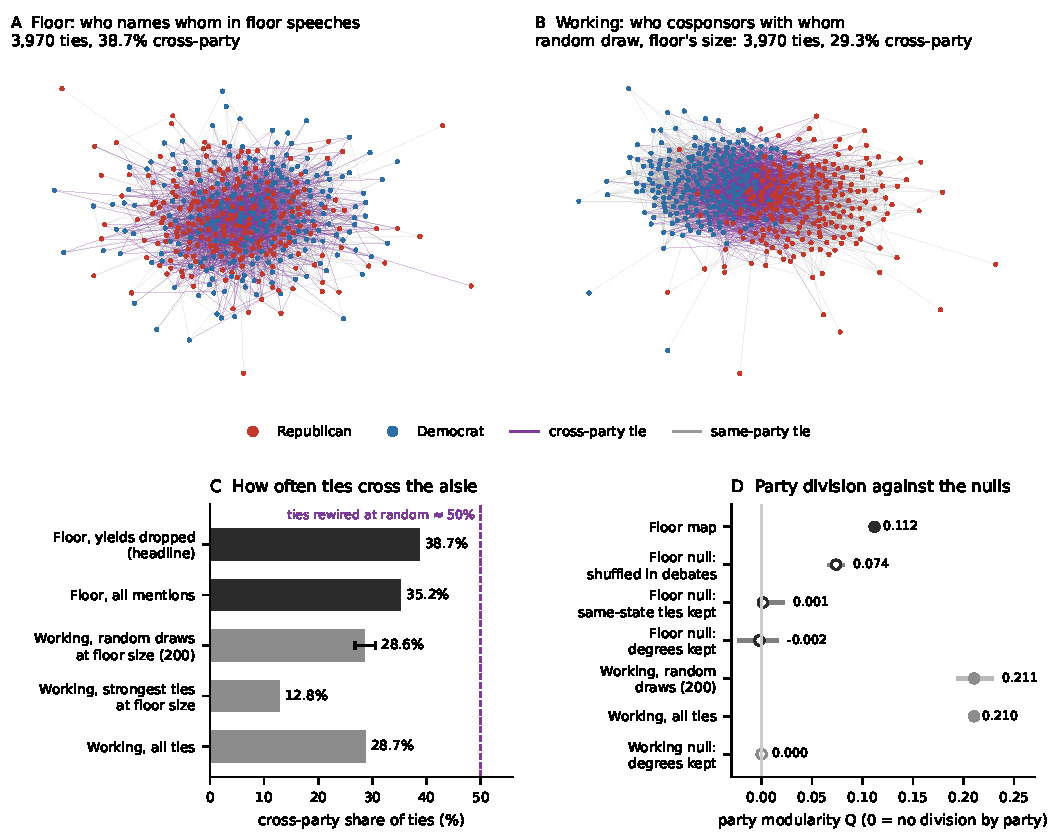
\includegraphics[width=17.8cm]{figures/figure1.pdf}
% Generated by report/md2tex.py from Martin/results_part1.md. Do not edit by hand.
\caption{The House as two networks, January 2025 to November 2026. (\emph{A}) Floor map: members tied when one names the other in a floor speech, yields of debate time left out. (\emph{B}) Working map: one random draw of sponsor–cosponsor ties, thinned to the floor map's 3,970 ties. Nodes are members (red Republican, blue Democrat); purple ties cross the aisle. Positions come from a spring layout and carry no meaning. (\emph{C}) Share of ties that cross the aisle; the bar for the random draws shows the range over 200 draws, and the dashed line the level expected if ties were rewired at random. (\emph{D}) Party modularity of each map (filled) against its nulls (open; lines show the range over the draws): shuffling who is named within each debate, keeping each member's same-state ties, and keeping each member's number of ties.}

\label{fig:maps}
\end{figure*}

\subsection*{What a cross-party mention means}

Naming a colleague is not working with them, and a member can name the other side to attack it. To find out what
the floor map's cross-party ties are, we read 100 floor mentions drawn at random, 75 between parties and 25 within
a party, and coded what the speaker was doing towards the named member (Methods). Of the cross-party mentions, 69\%
(95\% interval 58\% to 79\%) were agreeing: thanks to a bill's co-lead or to a committee's chair, praise for joint
work, support for the member's bill. 23\% (15\% to 33\%) were neutral references, such as the member who
introduced a bill or whose district a constituent lives in. Only 7\% (3\% to 15\%) disagreed with the named member
(Fig.~\ref{fig:labels}). None was procedure: handing over debate time stays within a party (12\% of same-party
mentions). Two coders agreed on 82\% of the mentions (Cohen's $\kappa = 0.64$).

A text classifier trained on these labels could not carry them to all 9,909 floor mentions. Predicting each label
from a model trained on the other 99, it was right 73\% of the time, against 72\% for always answering
``agreeing'', and it found none of the five disagreements. We therefore report the hand-labelled shares only.

The floor map's cross-party ties are thus mostly acknowledgement, not argument. Members name the other side to
credit it far more often than to oppose it. The labels check that each name is the right member, but not which
members were missed: in 30 turns read in full, the matcher found 12 of the 13 members a reader found.

\begin{figure}[t]
\centering
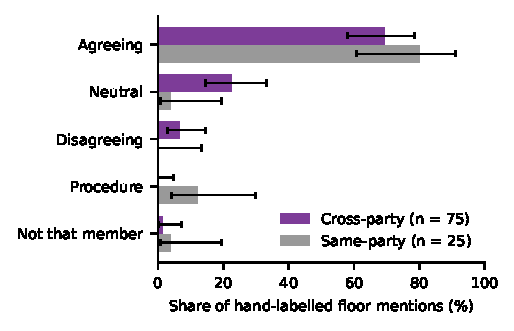
\includegraphics[width=8.7cm]{figures/figure2.pdf}
\caption{What floor mentions do. Share of 100 hand-labelled mentions in each code, for mentions between parties
(purple, $n = 75$) and within a party (grey, $n = 25$). Lines show 95\% Wilson intervals. Codes as in Methods; a
mention was coded ``not that member'' when the matched name referred to someone else.}
\label{fig:labels}
\end{figure}

\subsection*{Close-up: whom members name at home}
% Results, part 3: whom members name at home. Anas (with Claude), rewritten Mon 23 Nov 2026 (evening) at full length,
% after checks T and I (a4/CHECKS_PLAN_23NOV.md, designs fixed before running). One aim, with the detours kept:
% where the text count, the network, A5 and the checks disagree, the disagreement is stated and discussed.
% NOT cut to the word budget on purpose: every layer is here for the group's read-through (Wed 25 Nov), which decides
% what stays. Paragraphs marked [G17] are the optional extensions (home map, A5) the group still has to accept.
%
% Sources (all on the 22 Nov rerun; frozen inputs bc1c2344):
%   P1-P2  a4/out/results.csv, member_shares.csv, leave_one_state_out.csv; Figure 3. Range 7.9-10.1% = Figure 3A's
%          5-point bands beyond 5 points of own-party lean (bands with >= 5 members).
%   P3     check T: a4/check_tone/scored.csv (a4/README.md, "Check T").
%   P4     check I: a4/out/ideology_check.csv (a4/README.md, "Check I"); bands from members.csv nominate_dim1.
%   P5     home map: a4/out/home_measures_centrality.csv, home_measures_null.csv, home_ties.csv, alpha_centrality.csv
%          (a4/NETWORK_METHODS.md 3a, 3d).
%   P6     A5: a5/out/results.csv, a5/check/scored.csv, a5/mirror/scored.csv (a5/README.md).
% Martin's M6 paragraph (% Generated by report/md2tex.py from Martin/results_part1.md. Do not edit by hand.
\textbf{Do members show their cross-party bills at home?} Of the bills a member sponsored, those with an original cosponsor from the other party were cited in that member's press releases more often than their other bills (52.7\% against 45.1\%; 388 members, 10,125 bills). Shuffling, within each member, which bills count as cross-party gives a null in which the observed count is 1.08 times the expected (p < 0.001), in both parties. Most of the gap, however, separates co-led bills from solo bills: against bills co-led only by the member's own party, cross-party bills are cited 3.5 points more often (52.6\% against 49.1\%, p = 0.02). As original cosponsors, members cite the cross-party bills they join about three times as often as same-party ones (8.6\% against 2.9\%). We cannot rule out that bipartisan bills are cited more because they more often pass.
) follows this file in results.tex.
% To use: replace the placeholder under "Close-up" in report/sections/results.tex with % Results, part 3: whom members name at home. Anas (with Claude), rewritten Mon 23 Nov 2026 (evening) at full length,
% after checks T and I (a4/CHECKS_PLAN_23NOV.md, designs fixed before running). One aim, with the detours kept:
% where the text count, the network, A5 and the checks disagree, the disagreement is stated and discussed.
% NOT cut to the word budget on purpose: every layer is here for the group's read-through (Wed 25 Nov), which decides
% what stays. Paragraphs marked [G17] are the optional extensions (home map, A5) the group still has to accept.
%
% Sources (all on the 22 Nov rerun; frozen inputs bc1c2344):
%   P1-P2  a4/out/results.csv, member_shares.csv, leave_one_state_out.csv; Figure 3. Range 7.9-10.1% = Figure 3A's
%          5-point bands beyond 5 points of own-party lean (bands with >= 5 members).
%   P3     check T: a4/check_tone/scored.csv (a4/README.md, "Check T").
%   P4     check I: a4/out/ideology_check.csv (a4/README.md, "Check I"); bands from members.csv nominate_dim1.
%   P5     home map: a4/out/home_measures_centrality.csv, home_measures_null.csv, home_ties.csv, alpha_centrality.csv
%          (a4/NETWORK_METHODS.md 3a, 3d).
%   P6     A5: a5/out/results.csv, a5/check/scored.csv, a5/mirror/scored.csv (a5/README.md).
% Martin's M6 paragraph (% Generated by report/md2tex.py from Martin/results_part1.md. Do not edit by hand.
\textbf{Do members show their cross-party bills at home?} Of the bills a member sponsored, those with an original cosponsor from the other party were cited in that member's press releases more often than their other bills (52.7\% against 45.1\%; 388 members, 10,125 bills). Shuffling, within each member, which bills count as cross-party gives a null in which the observed count is 1.08 times the expected (p < 0.001), in both parties. Most of the gap, however, separates co-led bills from solo bills: against bills co-led only by the member's own party, cross-party bills are cited 3.5 points more often (52.6\% against 49.1\%, p = 0.02). As original cosponsors, members cite the cross-party bills they join about three times as often as same-party ones (8.6\% against 2.9\%). We cannot rule out that bipartisan bills are cited more because they more often pass.
) follows this file in results.tex.
% To use: replace the placeholder under "Close-up" in report/sections/results.tex with % Results, part 3: whom members name at home. Anas (with Claude), rewritten Mon 23 Nov 2026 (evening) at full length,
% after checks T and I (a4/CHECKS_PLAN_23NOV.md, designs fixed before running). One aim, with the detours kept:
% where the text count, the network, A5 and the checks disagree, the disagreement is stated and discussed.
% NOT cut to the word budget on purpose: every layer is here for the group's read-through (Wed 25 Nov), which decides
% what stays. Paragraphs marked [G17] are the optional extensions (home map, A5) the group still has to accept.
%
% Sources (all on the 22 Nov rerun; frozen inputs bc1c2344):
%   P1-P2  a4/out/results.csv, member_shares.csv, leave_one_state_out.csv; Figure 3. Range 7.9-10.1% = Figure 3A's
%          5-point bands beyond 5 points of own-party lean (bands with >= 5 members).
%   P3     check T: a4/check_tone/scored.csv (a4/README.md, "Check T").
%   P4     check I: a4/out/ideology_check.csv (a4/README.md, "Check I"); bands from members.csv nominate_dim1.
%   P5     home map: a4/out/home_measures_centrality.csv, home_measures_null.csv, home_ties.csv, alpha_centrality.csv
%          (a4/NETWORK_METHODS.md 3a, 3d).
%   P6     A5: a5/out/results.csv, a5/check/scored.csv, a5/mirror/scored.csv (a5/README.md).
% Martin's M6 paragraph (\input{sections/from_martin_m6}) follows this file in results.tex.
% To use: replace the placeholder under "Close-up" in report/sections/results.tex with \input{sections/results_part3}.
% About 930 words after the humanizer pass (23 Nov); every number of the earlier version kept. Cuts: Wednesday.

\textbf{Members in exposed seats name the other party more often at home, in both parties.} We asked whom members name in their own press releases, and whether members whose seat is at risk name the other party more. For each of the 406 members with at least ten releases (53,664 releases, 3 January 2025 to 20 November 2026), we measured the share of releases naming a House member of the other party who is neither a party leader nor a co-lead of a bill the release cites. A seat is exposed when the district the member served leans toward their own party by five points or less (Cook PVI 2025). Exposed Republicans named Democrats in 13.3\% of their releases, against 9.2\% for safe Republicans; exposed Democrats named Republicans in 11.6\%, against 9.0\% (permutation $p = 0.004$ for each; Fig.~\ref{fig:home}). The two gaps differ by 1.5 points ($p = 0.36$), too little to tell whether being in the president's party matters.

\textbf{The difference sits in the closest seats.} Members whose district is even or leans to the other party named the other party most (Republicans 19.2\%, $n = 8$; Democrats 14.2\%, $n = 10$). Beyond five points of lean the share is nearly flat, between 7.9\% and 10.1\% (Fig.~\ref{fig:home}\emph{A}). Every check fixed before the analysis gives a positive gap in both parties with $p < 0.05$: other cut-offs, the 2024 presidential margin instead of Cook, leaving out the 21 members whose label changes or is unknown under the 2026 maps, leaving out releases about redistricting or caucuses, and the floor's matcher without the press additions (Fig.~\ref{fig:home}\emph{B}). The gaps keep their sign when any one state is left out, and widen to 7.0 and 6.3 points when co-leads count too.

\textbf{Most of the names are partners.} A count says nothing about tone, and an exposed member could name the other side to attack it. Three blind AI readers, who did not see the seat, coded 60 counted names, 15 for each party and seat: 46 named a partner or praised the member (77\%), 9 were neutral mentions such as a committee chair addressed in a letter, 4 were wrong matches, and one criticised (a safe Republican on a Democrat's remarks). Exposed and safe seats did not differ in criticism. At home, as on the floor, cross-party names are mostly acknowledgement.

\textbf{Exposed members are also their party's moderates, and the two cannot be separated.} Of the 37 exposed Republicans, 22 are in their party's most moderate fifth by DW-NOMINATE, as are 27 of the 54 exposed Democrats; the most extreme fifths hold 3 and 2. Shuffling the exposed label only among members of the same party and ideology band gives the gap ideology alone would produce: 2.9 of the 4.1 Republican points and 2.4 of the 2.6 Democratic points. The remainder (1.1 and 0.2 points) cannot be told from chance ($p = 0.39$ and $0.76$), so our data cannot say whether the seat or the member's ideology drives the naming. The test is strict: DW-NOMINATE comes from roll-call votes, and members may vote moderately because their seat is close, so holding it fixed can remove part of a real seat effect. More of the Republican gap survives, a party difference that returns in the network.

% [G17] Home map (network extension): keep or cut on Wednesday. Its comparisons inherit the ideology caveat (not tested).
% If kept: the 'majority's control of committees' clause is untested. Possible test, decided 23 Nov to wait for Wednesday:
% sort counted cross-party names by route (same committee / bill release / other), exposed vs safe by party
% (Martin/m5_committees, a3 bill links), design written first, labelled exploratory. About 1.5 h. See a4/README.md.
\textbf{The network sees the two parties differently.} Tying two members when one names the other gives a home map of the same 406 members. In both parties exposed members are its hubs: they are 22\% of members but send 35\% and receive 34\% of its cross-party ties, and are tied to 1.9 times (Republicans) and 1.5 times (Democrats) as many members of the other party as safe members are (Holm-corrected $p = 0.001$ for each). On the backbone, which keeps each member's strongest ties, the parties split. Exposed Republicans have 1.5 times the backbone ties of safe Republicans (Holm $p = 0.013$), with borderline higher betweenness and closeness (Holm $p = 0.059$ and $0.055$): they bridge by volume. Exposed Democrats have as many backbone ties and as central a position as safe Democrats, but sit on more shortest paths than their ties predict (Holm $p = 0.08$ at our backbone level, below 0.05 at every looser one): they bridge by position. So one gap in the text hides two roles in the network. We did not test why; one possibility is that the majority's control of committees and the floor agenda gives exposed Republicans more occasions to name Democrats. Exposed members tie to each other only slightly more than their activity predicts (10.7\% of cross-party ties join two exposed members, against 10.2\% when ties are rewired with every member's number of ties kept; $p = 0.015$).

% [G17] A5 ("bipartisan"): keep or cut on Wednesday. Not tested against ideology.
\textbf{The word ``bipartisan'' mostly comes with a partner, and here the parties swap.} A quarter of the releases (13,744) call something bipartisan. In 64\% of them a House member of the other party is named or co-leads a cited bill, against 9\% of other releases (means over 370 members). Three blind AI readers checked 30 releases of each kind: of those naming a member of the other party, 28 named a partner and none an opponent; of those naming none, 29 named no partner from the other party and one named a senator, whom our matcher does not count. By seat, the difference runs the other way from the backbone: exposed Democrats back the word with a partner more often than safe Democrats (63.0\% against 56.7\%, $p = 0.012$), while exposed and safe Republicans do not differ (72.1\% against 69.1\%, $p = 0.40$) and both exceed Democrats (not tested).
.
% About 930 words after the humanizer pass (23 Nov); every number of the earlier version kept. Cuts: Wednesday.

\textbf{Members in exposed seats name the other party more often at home, in both parties.} We asked whom members name in their own press releases, and whether members whose seat is at risk name the other party more. For each of the 406 members with at least ten releases (53,664 releases, 3 January 2025 to 20 November 2026), we measured the share of releases naming a House member of the other party who is neither a party leader nor a co-lead of a bill the release cites. A seat is exposed when the district the member served leans toward their own party by five points or less (Cook PVI 2025). Exposed Republicans named Democrats in 13.3\% of their releases, against 9.2\% for safe Republicans; exposed Democrats named Republicans in 11.6\%, against 9.0\% (permutation $p = 0.004$ for each; Fig.~\ref{fig:home}). The two gaps differ by 1.5 points ($p = 0.36$), too little to tell whether being in the president's party matters.

\textbf{The difference sits in the closest seats.} Members whose district is even or leans to the other party named the other party most (Republicans 19.2\%, $n = 8$; Democrats 14.2\%, $n = 10$). Beyond five points of lean the share is nearly flat, between 7.9\% and 10.1\% (Fig.~\ref{fig:home}\emph{A}). Every check fixed before the analysis gives a positive gap in both parties with $p < 0.05$: other cut-offs, the 2024 presidential margin instead of Cook, leaving out the 21 members whose label changes or is unknown under the 2026 maps, leaving out releases about redistricting or caucuses, and the floor's matcher without the press additions (Fig.~\ref{fig:home}\emph{B}). The gaps keep their sign when any one state is left out, and widen to 7.0 and 6.3 points when co-leads count too.

\textbf{Most of the names are partners.} A count says nothing about tone, and an exposed member could name the other side to attack it. Three blind AI readers, who did not see the seat, coded 60 counted names, 15 for each party and seat: 46 named a partner or praised the member (77\%), 9 were neutral mentions such as a committee chair addressed in a letter, 4 were wrong matches, and one criticised (a safe Republican on a Democrat's remarks). Exposed and safe seats did not differ in criticism. At home, as on the floor, cross-party names are mostly acknowledgement.

\textbf{Exposed members are also their party's moderates, and the two cannot be separated.} Of the 37 exposed Republicans, 22 are in their party's most moderate fifth by DW-NOMINATE, as are 27 of the 54 exposed Democrats; the most extreme fifths hold 3 and 2. Shuffling the exposed label only among members of the same party and ideology band gives the gap ideology alone would produce: 2.9 of the 4.1 Republican points and 2.4 of the 2.6 Democratic points. The remainder (1.1 and 0.2 points) cannot be told from chance ($p = 0.39$ and $0.76$), so our data cannot say whether the seat or the member's ideology drives the naming. The test is strict: DW-NOMINATE comes from roll-call votes, and members may vote moderately because their seat is close, so holding it fixed can remove part of a real seat effect. More of the Republican gap survives, a party difference that returns in the network.

% [G17] Home map (network extension): keep or cut on Wednesday. Its comparisons inherit the ideology caveat (not tested).
% If kept: the 'majority's control of committees' clause is untested. Possible test, decided 23 Nov to wait for Wednesday:
% sort counted cross-party names by route (same committee / bill release / other), exposed vs safe by party
% (Martin/m5_committees, a3 bill links), design written first, labelled exploratory. About 1.5 h. See a4/README.md.
\textbf{The network sees the two parties differently.} Tying two members when one names the other gives a home map of the same 406 members. In both parties exposed members are its hubs: they are 22\% of members but send 35\% and receive 34\% of its cross-party ties, and are tied to 1.9 times (Republicans) and 1.5 times (Democrats) as many members of the other party as safe members are (Holm-corrected $p = 0.001$ for each). On the backbone, which keeps each member's strongest ties, the parties split. Exposed Republicans have 1.5 times the backbone ties of safe Republicans (Holm $p = 0.013$), with borderline higher betweenness and closeness (Holm $p = 0.059$ and $0.055$): they bridge by volume. Exposed Democrats have as many backbone ties and as central a position as safe Democrats, but sit on more shortest paths than their ties predict (Holm $p = 0.08$ at our backbone level, below 0.05 at every looser one): they bridge by position. So one gap in the text hides two roles in the network. We did not test why; one possibility is that the majority's control of committees and the floor agenda gives exposed Republicans more occasions to name Democrats. Exposed members tie to each other only slightly more than their activity predicts (10.7\% of cross-party ties join two exposed members, against 10.2\% when ties are rewired with every member's number of ties kept; $p = 0.015$).

% [G17] A5 ("bipartisan"): keep or cut on Wednesday. Not tested against ideology.
\textbf{The word ``bipartisan'' mostly comes with a partner, and here the parties swap.} A quarter of the releases (13,744) call something bipartisan. In 64\% of them a House member of the other party is named or co-leads a cited bill, against 9\% of other releases (means over 370 members). Three blind AI readers checked 30 releases of each kind: of those naming a member of the other party, 28 named a partner and none an opponent; of those naming none, 29 named no partner from the other party and one named a senator, whom our matcher does not count. By seat, the difference runs the other way from the backbone: exposed Democrats back the word with a partner more often than safe Democrats (63.0\% against 56.7\%, $p = 0.012$), while exposed and safe Republicans do not differ (72.1\% against 69.1\%, $p = 0.40$) and both exceed Democrats (not tested).
.
% About 930 words after the humanizer pass (23 Nov); every number of the earlier version kept. Cuts: Wednesday.

\textbf{Members in exposed seats name the other party more often at home, in both parties.} We asked whom members name in their own press releases, and whether members whose seat is at risk name the other party more. For each of the 406 members with at least ten releases (53,664 releases, 3 January 2025 to 20 November 2026), we measured the share of releases naming a House member of the other party who is neither a party leader nor a co-lead of a bill the release cites. A seat is exposed when the district the member served leans toward their own party by five points or less (Cook PVI 2025). Exposed Republicans named Democrats in 13.3\% of their releases, against 9.2\% for safe Republicans; exposed Democrats named Republicans in 11.6\%, against 9.0\% (permutation $p = 0.004$ for each; Fig.~\ref{fig:home}). The two gaps differ by 1.5 points ($p = 0.36$), too little to tell whether being in the president's party matters.

\textbf{The difference sits in the closest seats.} Members whose district is even or leans to the other party named the other party most (Republicans 19.2\%, $n = 8$; Democrats 14.2\%, $n = 10$). Beyond five points of lean the share is nearly flat, between 7.9\% and 10.1\% (Fig.~\ref{fig:home}\emph{A}). Every check fixed before the analysis gives a positive gap in both parties with $p < 0.05$: other cut-offs, the 2024 presidential margin instead of Cook, leaving out the 21 members whose label changes or is unknown under the 2026 maps, leaving out releases about redistricting or caucuses, and the floor's matcher without the press additions (Fig.~\ref{fig:home}\emph{B}). The gaps keep their sign when any one state is left out, and widen to 7.0 and 6.3 points when co-leads count too.

\textbf{Most of the names are partners.} A count says nothing about tone, and an exposed member could name the other side to attack it. Three blind AI readers, who did not see the seat, coded 60 counted names, 15 for each party and seat: 46 named a partner or praised the member (77\%), 9 were neutral mentions such as a committee chair addressed in a letter, 4 were wrong matches, and one criticised (a safe Republican on a Democrat's remarks). Exposed and safe seats did not differ in criticism. At home, as on the floor, cross-party names are mostly acknowledgement.

\textbf{Exposed members are also their party's moderates, and the two cannot be separated.} Of the 37 exposed Republicans, 22 are in their party's most moderate fifth by DW-NOMINATE, as are 27 of the 54 exposed Democrats; the most extreme fifths hold 3 and 2. Shuffling the exposed label only among members of the same party and ideology band gives the gap ideology alone would produce: 2.9 of the 4.1 Republican points and 2.4 of the 2.6 Democratic points. The remainder (1.1 and 0.2 points) cannot be told from chance ($p = 0.39$ and $0.76$), so our data cannot say whether the seat or the member's ideology drives the naming. The test is strict: DW-NOMINATE comes from roll-call votes, and members may vote moderately because their seat is close, so holding it fixed can remove part of a real seat effect. More of the Republican gap survives, a party difference that returns in the network.

% [G17] Home map (network extension): keep or cut on Wednesday. Its comparisons inherit the ideology caveat (not tested).
% If kept: the 'majority's control of committees' clause is untested. Possible test, decided 23 Nov to wait for Wednesday:
% sort counted cross-party names by route (same committee / bill release / other), exposed vs safe by party
% (Martin/m5_committees, a3 bill links), design written first, labelled exploratory. About 1.5 h. See a4/README.md.
\textbf{The network sees the two parties differently.} Tying two members when one names the other gives a home map of the same 406 members. In both parties exposed members are its hubs: they are 22\% of members but send 35\% and receive 34\% of its cross-party ties, and are tied to 1.9 times (Republicans) and 1.5 times (Democrats) as many members of the other party as safe members are (Holm-corrected $p = 0.001$ for each). On the backbone, which keeps each member's strongest ties, the parties split. Exposed Republicans have 1.5 times the backbone ties of safe Republicans (Holm $p = 0.013$), with borderline higher betweenness and closeness (Holm $p = 0.059$ and $0.055$): they bridge by volume. Exposed Democrats have as many backbone ties and as central a position as safe Democrats, but sit on more shortest paths than their ties predict (Holm $p = 0.08$ at our backbone level, below 0.05 at every looser one): they bridge by position. So one gap in the text hides two roles in the network. We did not test why; one possibility is that the majority's control of committees and the floor agenda gives exposed Republicans more occasions to name Democrats. Exposed members tie to each other only slightly more than their activity predicts (10.7\% of cross-party ties join two exposed members, against 10.2\% when ties are rewired with every member's number of ties kept; $p = 0.015$).

% [G17] A5 ("bipartisan"): keep or cut on Wednesday. Not tested against ideology.
\textbf{The word ``bipartisan'' mostly comes with a partner, and here the parties swap.} A quarter of the releases (13,744) call something bipartisan. In 64\% of them a House member of the other party is named or co-leads a cited bill, against 9\% of other releases (means over 370 members). Three blind AI readers checked 30 releases of each kind: of those naming a member of the other party, 28 named a partner and none an opponent; of those naming none, 29 named no partner from the other party and one named a senator, whom our matcher does not count. By seat, the difference runs the other way from the backbone: exposed Democrats back the word with a partner more often than safe Democrats (63.0\% against 56.7\%, $p = 0.012$), while exposed and safe Republicans do not differ (72.1\% against 69.1\%, $p = 0.40$) and both exceed Democrats (not tested).


% Generated by report/md2tex.py from Martin/results_part1.md. Do not edit by hand.
\textbf{Do members show their cross-party bills at home?} Of the bills a member sponsored, those with an original cosponsor from the other party were cited in that member's press releases more often than their other bills (52.7\% against 45.1\%; 388 members, 10,125 bills). Shuffling, within each member, which bills count as cross-party gives a null in which the observed count is 1.08 times the expected (p < 0.001), in both parties. Most of the gap, however, separates co-led bills from solo bills: against bills co-led only by the member's own party, cross-party bills are cited 3.5 points more often (52.6\% against 49.1\%, p = 0.02). As original cosponsors, members cite the cross-party bills they join about three times as often as same-party ones (8.6\% against 2.9\%). We cannot rule out that bipartisan bills are cited more because they more often pass.


\begin{figure}[t]
\centering
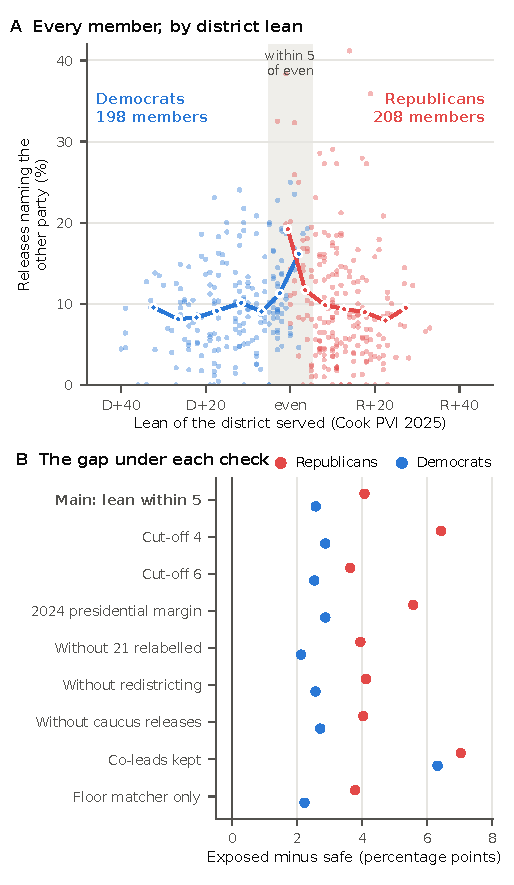
\includegraphics[width=8.7cm]{figures/figure3.pdf}
\caption{\textbf{Members in exposed seats name the other party more often in their press releases.} (\emph{A}) Each dot is one of 406 House members (198 Democrats, 208 Republicans; 53,664 releases, 3 January 2025 to 20 November 2026): the share of their releases that name a House member of the other party who is neither a party leader nor a co-lead of a bill the release cites, against the lean of the district they served (Cook PVI 2025). Lines join the mean share in 5-point bands of lean (bands with at least five members). Shading marks districts within five points of even; a member counts as exposed when the district leans toward their own party by five points or less, which includes seats leaning to the other party. (\emph{B}) Exposed minus safe mean share, by party, for the main definition (top) and for each check fixed before the analysis: other cut-offs, the 2024 presidential margin as lean, leaving out the 21 members relabelled or unplaced under the 2026 maps, leaving out releases about redistricting or caucuses, counting co-leads, and the floor's matcher without the press additions. Every gap is positive with $p < 0.05$ (labels shuffled within party, 10,000 shuffles).}
\label{fig:home}
\end{figure}
